\documentclass[tikz]{standalone}
\usepackage{pgfplots}
\pgfplotsset{compat=1.15}
\usepackage{mathrsfs}
\usetikzlibrary{arrows,calc}
\usepackage{tkz-euclide}

\usepackage{fp}
\pagestyle{empty}

\definecolor{AngleClr}{rgb}{0,0.39215686274509803,0}
\definecolor{ShapeClr}{rgb}{0.6,0.2,0}
\definecolor{BlueClr}{RGB}{5,81,163}

\begin{document}

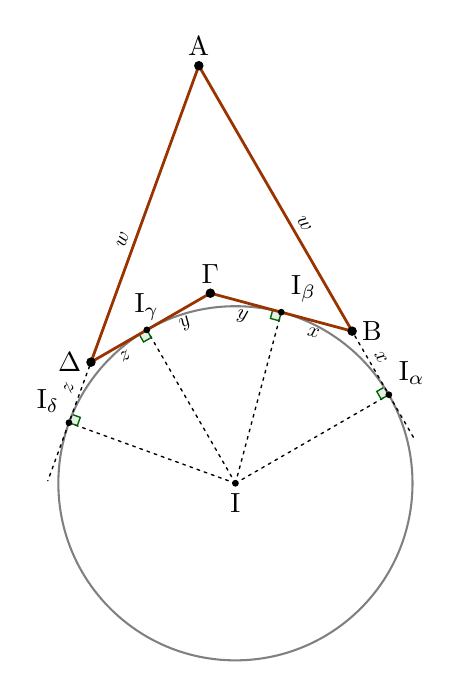
\begin{tikzpicture}[scale=.75]
\tkzSetUpLine[line width=1pt,color=black]
\tkzSetUpPoint[fill=black]

\tkzDefPoints{0/0/I}

% Define the points where the circle touches the quadrilateral.
\tkzDefPoint(30:3){Ia}
\tkzDefPoint(75:3){Ib}
\tkzDefPoint(120:3){Ic}
\tkzDefPoint(160:3){Id}

% Find the lines containing the sides of the quadrilateral.
\tkzDefLine[tangent at=Ia](I) \tkzGetPoint{h1}
\tkzDefLine[tangent at=Ib](I) \tkzGetPoint{h2}
\tkzDefLine[tangent at=Ic](I) \tkzGetPoint{h3}
\tkzDefLine[tangent at=Id](I) \tkzGetPoint{h4}


\tkzDrawSegments[line width=0.5pt,color=black,dashed,dash pattern=on 1pt off 1.75pt](I,Ia I,Ib I,Ic I,Id)


% Find the vertices of the quadrilateral.
\tkzInterLL(Id,h4)(Ia,h1)\tkzGetPoint{A}
\tkzInterLL(Ia,h1)(Ib,h2)\tkzGetPoint{B}
\tkzInterLL(Ib,h2)(Ic,h3)\tkzGetPoint{C}
\tkzInterLL(Ic,h3)(Id,h4)\tkzGetPoint{D}

\tkzMarkRightAngles[line width=0.5pt, size=.15,color=AngleClr,fill=AngleClr,fill opacity=0.1](I,Ia,B I,Ib,C I,Ic,D I,Id,A)

\tkzDrawCircle[line width=0.75](I,Ia)


% Draw the quadrilateral.
\tkzDrawSegments[line width=0.5pt,color=black,dashed,dash pattern=on 1pt off 1.75pt,add=0 and 0.4](A,D A,B)
\tkzFillPolygon[fill=white,fill opacity=0.1](A,B,C,D)
\tkzDrawPolygon[color=ShapeClr](A,B,C,D)

\tkzDrawPoints[size=3](A,B,C,D)
\tkzDrawPoints[size=2](Ia,Ib,Ic,Id,I)
\tkzLabelPoint[above right](Ia){${\rm I}_\alpha$}
\tkzLabelPoint[above right](Ib){${\rm I}_\beta$}
\tkzLabelPoint[above](Ic){${\rm I}_\gamma$}
\tkzLabelPoint[above left](Id){${\rm I}_\delta$}
\tkzLabelPoint[below](I){$\rm I$}

\tkzLabelPoint[above](A){$\rm A$}
\tkzLabelPoint[right](B){$\rm B$}
\tkzLabelPoint[above](C){$\rm \Gamma$}
\tkzLabelPoint[left](D){$\rm \Delta$}

\tkzLabelSegments[above,sloped,scale=0.75](A,Id A,Ia){$w$}
\tkzLabelSegments[above,sloped,scale=0.75](B,Ia){$x$}
\tkzLabelSegments[below,sloped,scale=0.75](B,Ib){$x$}
\tkzLabelSegments[below,sloped,scale=0.75](C,Ib C,Ic){$y$}
\tkzLabelSegments[below,sloped,scale=0.75](D,Ic){$z$}
\tkzLabelSegments[above,sloped,scale=0.75](D,Id){$z$}

\end{tikzpicture}

\end{document}
